\documentclass[11pt]{book}
\usepackage[colorlinks = true,linkcolor = blue]{hyperref}
\usepackage[letterpaper]{geometry} % Custom margins
\usepackage{graphicx}
\usepackage{tabularx}
\usepackage{float}
\usepackage[spanish]{babel}
\usepackage[T1]{fontenc}
\usepackage[utf8]{inputenc}
\usepackage{remreset}
\usepackage{enumitem}
\usepackage{xparse}
\usepackage{wrapfig}
\usepackage{amssymb,amsmath}
\usepackage{tikz}
\usetikzlibrary{
  arrows,
  positioning,
  matrix,
  calc,
  decorations.pathreplacing,
  decorations.pathmorphing,
  decorations.markings,
  decorations.text,
  shapes,
  backgrounds,
  shadows,
  trees,
  fit,
  snakes,
  patterns,
  mindmap,
  intersections,
  calendar,
  plotmarks,
  spy,
  tikzmark}
  
  \decimalpoint

%%%% APRENDISAJES TEXTBOX
\tikzset{
  abstractbox/.style={
    draw=black, fill=white, rectangle, 
    inner sep=12pt, style=rounded corners,
    drop shadow={fill=black, opacity=1}
  },
  abstracttitle/.style={fill=white}
}
\newcommand{\boxabstract}[2][fill=white]{
  \begin{tikzpicture}
    \node [abstractbox, #1] (box)
    {\begin{minipage}{0.9\linewidth}
        \setlength{\parindent}{2mm} % Indentar.
        \normalfont #2
      \end{minipage}};
    \node[abstracttitle, right=10pt] at (box.north west) {Aprendizajes esperados:};
    \node[draw=none, fit=(box)] {};
  \end{tikzpicture}
}
%%%%%%%%%%%%%%%%%%%%%%%%

\makeatletter
  \@removefromreset{section}{chapter}
\makeatother
\addto\captionsspanish{\renewcommand{\chaptername}{}}
\renewcommand{\thechapter}{Unidad \arabic{chapter}}
\renewcommand{\thesection}{S\arabic{section}}
\renewcommand{\thesubsection}{L\arabic{subsection}}
\setlength{\parindent}{0pt}

%%%%%%%%%%%%% START questions env
%Idea from https://tex.stackexchange.com/a/236668/1952
\DeclareDocumentCommand\question{o}{%
    \item\IfNoValueTF{#1}{}{(#1 puntos)}}
\newenvironment{questions}[1][]{\enumerate[,#1]}{\endenumerate}
\newlist{oneparchoices}{enumerate*}{1}
\setlist[oneparchoices,1]{label=\quad\alph*), itemjoin={{\quad}}}
\newlist{choices}{enumerate*}{1}
\setlist[choices,1]{label=\quad$\square$, itemjoin={{\\}},leftmargin = 1cm}
\newcommand{\choice}{\item}
%%%%%%%%%%%%% END questions env
\makeatletter
  \@removefromreset{section}{chapter}
\makeatother

\begin{document}
\pagestyle{empty}
\newgeometry{letterpaper,left=15mm,top=50mm,bottom=0mm} % Custom margins
\begin{center}
  {\Huge Matem\'aticas 3}\\
  \vspace{2cm}
  \normalsize
  \textbf{\large Cuaderno de trabajo}\\
  para los alumnos de 3$^\circ$ de  Secundaria\\
  en el curso durante el ciclo escolar\\
  \textbf{2022-2023}\\
  \vspace{2.5cm}
  \small POR\\
  \Large J. C. Melchor Pinto\\[0.5em]
  \normalsize Profesor de asignatura en\\
  \vspace{1cm}
  
\includegraphics[width=4cm]{./Unidad 2/Images/LOGO_RDS_nobg}
\end{center}
\vspace{2cm}
%\include*{Functional/TitlePage}
\hspace{-16mm}
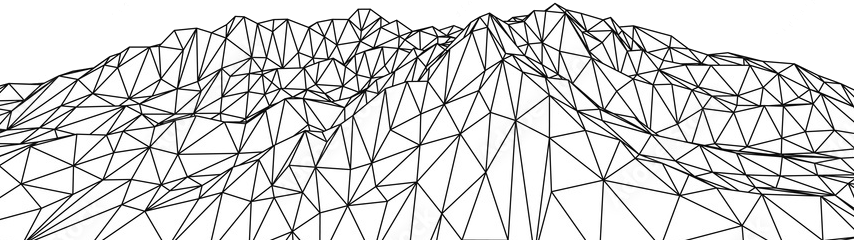
\includegraphics[width=\paperwidth]{./Unidad 2/Images/cover_bg}
\restoregeometry
\tableofcontents
\chapter{}

\section{Múltiplos y divisores}
\subsection{Múltiplos}
\subsection{Divisores}
\subsection{Problemas de multiplicación y división de fracciones}
\subsection{Multiplicación de números positivos y negativos}

\section{Números primos}
\subsection{Números primos y compuestos}
\subsection{Factorización y descomposición en números primos}

\section{Mínimo común múltiplo y máximo común divisor}
\subsection{Mínimo común múltiplo}
\subsection{Máximo común divisor}

\section{Polígonos semejantes}
\subsection{Semejanza de polígonos}
\subsection{Construcción de polígonos semejantes}

\section{Criterios de semejanza de triángulos}
\subsection{Criterios de semejanza de triángulos}
\subsection{Aplicaciones de semejanza de triángulos}

\section{Medidas de tendencia central y de dispersión}
\subsection{Significado de las medidas de tendencia central}
\subsection{Significado de las medidas de dispersión}
\subsection{Comparación de dos conjuntos de datos}


\chapter{}

\section{Ecuaciones cuadráticas}
\subsection{Ecuaciones cuadráticas}
\subsection{Gr\'aficas de expresiones cuadráticas y soluciones de sus ecuaciones}

\section{Resolución de ecuaciones cuadráticas}
\subsection{Procedimientos para la resolución de ecuaciones cuadráticas}
\subsection{Fórmula general de la ecuación de segundo grado}

\section{Relación entre variación y ecuación cuadrática}
\subsection{Variación cuadrática y ecuación asociada}
\subsection{Modelación de situaciones de variación cuadrática}

\section{Características de la variación}
\subsection{Distintos tipos de variación}
\subsection{Dependencia y razón de cambio}

\section{Análisis de la variación cuadrática}
\subsection{Representación tabular de la variación cuadrática}
\subsection{Representación algebraica de la variación cuadrática}
\subsection{Representación gr\'afica de la variación cuadrática}
\subsection{Representación tabular, algebraica y gr\'afica de variaciones cuadráticas}

\section{Variaciones diversas}
\subsection{Interpretación de gr\'aficas}
\subsection{Construcción de gr\'aficas a partir de tablas}
\subsection{Análisis de gr\'aficas de variaciones diversas}

\section{Eventos mutuamente excluyentes}
\subsection{Eventos singulares y no singulares}
\subsection{Eventos mutuamente excluyentes}
\subsection{Unión de dos eventos}
\subsection{Regla de la suma de probabilidades}

%%% U3
\chapter{}

\section{Expresiones algebraicas de segundo grado}
\subsection{Áreas y expresiones de segundo grado}
\subsection{Operaciones algebraicas}
\subsection{Factorización de expresiones de segundo grado}

\section{Expresiones algebraicas de ecuaciones y funciones}
\subsection{Expresiones algebraicas de ecuaciones}
\subsection{Expresiones algebraicas de funciones}

\section{Teorema de Pitágoras}
\subsection{Triángulos rectángulos y el teorema de Pitágoras}
\subsection{El teorema de Pitágoras}
\subsection{Aplicaciones del teorema de Pitágoras}

\section{Razones trigonométricas (seno, coseno y tangente)}
\subsection{Razones trigonométricas básicas}
\subsection{Razones trigonométricas de 30$^{\circ}$, 45$^{\circ}$ y 60$^{\circ}$}

\section{Resolución de triángulos rectángulos}
\subsection{Seno, coseno y tangente de ángulos agudos}
\subsection{Aplicaciones de razones trigonométricas}





\end{document}






